%The local system's analysis is very similar to the base station analysis. Comparing to the base station, this system doesn't implement the parking spaces detection, since it doesn't have a camera, and only communicates with the base station. As in the base station, one can say that this is a passive system since it is most of the time waiting for something to happen.
%
%\subsection{Events}
%Listed in the table below, table \ref{table:bs_events}, are the main events that will occur in the local system and will affect its behavior. 
%
%\begin{table}[h]
%	\centering
%	\resizebox{\columnwidth}{!}
%	{
%	\begin{tabular}{||c | c | c | c||} 
%		\hline
%		\textbf{Event} & \textbf{System Response} & \textbf{Source} & \textbf{Type}\\
%		\hline\hline
%Luminosity detector OFF & Power the lamp & Environment & Asynchronous\\\hline
%LED failure detector ON & Notify remote system & Local system & Asynchronous\\\hline
%Motion detected & Turn on the lamp & User & Asynchronous\\\hline
%Requested to turn on the lamp & Turn on the lamp & Base station & Asynchronous\\\hline
%Sensors data acquisition & Sample sensor values & Timer & Synchronous\\\hline
%Update system information & Send data to remote system & Base station & Asynchronous\\
%		\hline
%	\end{tabular}
%	}
%	
%	\caption{Local system events.}
%	\label{table:bs_events}
%\end{table}
%
%\subsection{Use Cases}
%The local system use cases are represented on figure \ref{fig:ls_use_cases}. Like the base station, a street passerby, can interact with the local system by moving in the vicinity of the lamppost, triggering it's motion detector.
%
%When movement is detected, the lamp is turned on and requests the base station to turn on the local system's neighbor lampposts. At the same time, the information that the lamppost was activated is sent to the base station, for this to be sent to the remote system.
%
%Also, the local system can be asked, by the base station, to turn on its lamp.
%\clearpage
%
%\begin{figure}[ht]
%	\centering
%	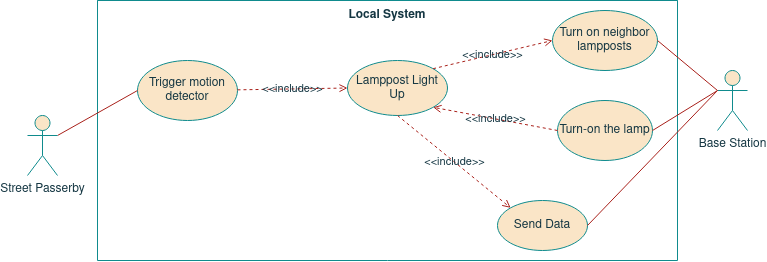
\includegraphics[width=1\textwidth]{/04local_system/LS_UseCase}
%	\caption{Local system use cases.}
%	\label{fig:ls_use_cases}
%\end{figure}
%
%\subsection{State Chart}
%In figure \ref{fig:ls_state_chart} is represented the state chart of the local system. After the system configuration, which initializes the Wi-Fi communication management, sensors data acquisition, the system enters an idle state. To do the sensors data acquisition, like in the base station, it is used a sample period, that periodically triggers the execution of the function “SampleSensors”, presented previously, in figure \ref{fig:sample_sensors}. When the local system is requested by the base station to turn on its lamp, the lamp is turned-on and a timeout is started (turn off time, as mentioned before). The lamppost status is then sent to the base station, in order to send it to the remote server.
%
%\begin{figure}[ht]
%	\centering
%	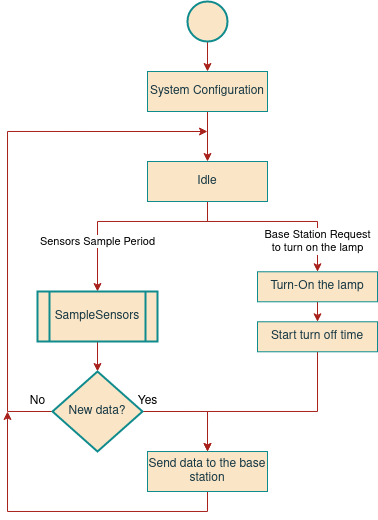
\includegraphics[width=.60\textwidth]{/04local_system/LS_StateChart}
%	\caption{Local system state chart.}
%	\label{fig:ls_state_chart}
%\end{figure}
%
%\clearpage
%\subsection{Sequence Diagram}
%The sequence diagram for the local system is represented in figure \ref{fig:ls_seq_diagram}. Again, this diagram is analogous to the one shown on the base station (figure \ref{fig:bs_seq_diagram}), having the differences that the local system only communicates with the base station, so any request that the local system wants to make to another local system has to go through the base station, and, due to that, the local system doesn't have the power to request another local system to turn its lamp on.
%
%\begin{figure}[ht]
%	\centering
%	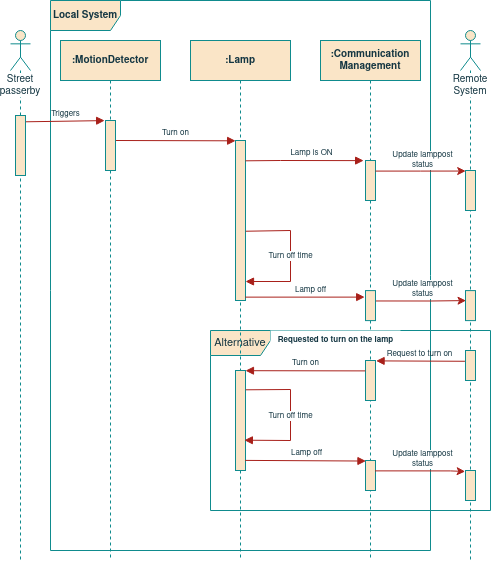
\includegraphics[width=.95\textwidth]{/04local_system/LS_SeqDiagram}
%	\caption{Local system sequence diagram.}
%	\label{fig:ls_seq_diagram}
%\end{figure}
